\documentclass{article}
\usepackage{graphicx}
\usepackage{amsmath}
\usepackage{hyperref}
\usepackage{cite}
\usepackage{listings}
\usepackage{xcolor}

\lstset{
    basicstyle=\ttfamily\small,
    keywordstyle=\color{blue},
    commentstyle=\color{gray},
    numbers=left,
    numberstyle=\tiny,
    stepnumber=1,
    breaklines=true,
    breakatwhitespace=false,
    columns=flexible,
}

\lstdefinelanguage{json}{
    basicstyle=\ttfamily\small,
    numbers=left,
    numberstyle=\tiny\color{gray},
    stepnumber=1,
    numbersep=5pt,
    showstringspaces=false,
    breaklines=true,
    frame=single,
    backgroundcolor=\color{gray!10},
    literate=
     *{0}{{{\color{blue}0}}}{1}
      {1}{{{\color{blue}1}}}{1}
      {2}{{{\color{blue}2}}}{1}
      {3}{{{\color{blue}3}}}{1}
      {4}{{{\color{blue}4}}}{1}
      {5}{{{\color{blue}5}}}{1}
      {6}{{{\color{blue}6}}}{1}
      {7}{{{\color{blue}7}}}{1}
      {8}{{{\color{blue}8}}}{1}
      {9}{{{\color{blue}9}}}{1},
}

\title{Utilizzo degli LLM per Generare Hugging Face Model Card da esempi di codice}
\author{Stefano Palombo}
\date{13 February 2025}

\begin{document}

\maketitle

\begin{abstract}
Negli ultimi anni, il rapido sviluppo del \textbf{machine learning} ha portato alla creazione di modelli sempre più avanzati e complessi, rendendo essenziale la disponibilità di strumenti che ne facilitino l’accesso e l’integrazione da parte degli sviluppatori.\\ 
Tra le piattaforme più influenti in questo ambito, \textbf{Hugging Face} si distingue per la sua vasta collezione di modelli open-source pre-addestrati (\textbf{PTM}) e per una community attiva nello sviluppo e documentazione dei modelli stessi. Ogni modello pubblicato è corredato da una \textbf{model card}, un documento che ne descrive le caratteristiche tecniche e i possibili casi d’uso, spesso accompagnato da esempi di codice Python per agevolarne l’implementazione.\\
L’obiettivo di questa tesi è analizzare la corrispondenza tra il codice presente nelle model card ufficiali di Hugging Face e l’effettivo utilizzo dei modelli in progetti open-source su GitHub. Per farlo, è stato adottato un approccio basato su data-mining, analisi del codice e generazione automatica di pattern mediante un \textbf{LLM} (Large Language Model).\\
Il primo passo è stato la raccolta e l’analisi di \textbf{141.749} script Python provenienti da repository pubblici, con lo scopo di estrarre file di codice che mostrassero l’uso pratico di \textbf{1024} modelli di Hugging Face. Questi snippet sono stati poi clusterizzati e filtrati per individuare pattern ricorrenti, che successivamente sono stati sintetizzati da un LLM, producendo 875 frammenti di codice rappresentativi. Parallelamente, è stato creato un dataset con gli snippet di codice presenti nelle model card ufficiali di Hugging Face, coprendo 751 modelli. Dopo aver intersecato questi dati con quelli prodotti dall’LLM, le \textbf{metriche di similarità} comunemente usate in letteratura, sono state calcolate per 625 modelli comuni.\\
Le analisi hanno evidenziato una similirità parziale pari al circa \textbf{40\%} dimostrandoche il codice generato dall’LLM non è una semplice copia del codice ufficiale, ma una sintesi alternativa basata su pattern più specifici, estratti direttamente dagli snippet reali\\.
Sebbene le metriche automatiche possano non sempre cogliere le somiglianze a livello concettuale, il codice generato dall’LLM può essere comunque utile per gli sviluppatori umani, che, attraverso un’analisi manuale, sono in grado di individuare dettagli tecnici rilevanti. Inoltre, per i modelli che non dispongono di esempi di codice nelle loro model card ufficiali, l’output generato dall’LLM potrebbe essere utilizzato come base per arricchire la documentazione, facilitando l’adozione dei modelli all’interno della community.\\
L’approccio sviluppato in questa tesi potrebbe, quindi, costituire un primo passo verso un sistema automatico di documentazione, in grado di \textbf{arricchire} le model card esistenti e fornire informazioni più dettagliate e contestualizzate sull’utilizzo reale dei modelli di Hugging Face, migliorando così l’\textbf{accessibilità} e la qualità.

\end{abstract}

\section{Introduzione}
Negli ultimi anni, il campo dell'intelligenza artificiale e in particolare del machine learning ha subito una crescita esponenziale portando allo sviluppo di modelli sempre più complessi e performanti.\\
Questo progresso ha reso necessario non soltanto il perfezionamento delle architetture dei modelli, ma anche la realizzazione di strumenti che ne facilitano l'accesso e l'implementazione da parte della community degli sviluppatori\\
Tra le varie piattaforme che rendono questi modelli più accessibili emerge \textbf{Hugging Face}\cite{huggingface}, che offre agli sviluppatori, tramite librerie open-source, la possibilità di sperimentarli per una vasta gamma di attività che spaziano tra la generazione e classificazione di testo naturale, classificazione di immagini, rilevezione di oggetti e molto altro.\\
L'utilità di Hugging Face non risiede soltanto nella disponibilità di modelli avanzati, ma anche nella sua community attiva, che contribuisce non solo nello sviluppo, ma anche alla documentazione dei modelli stessi. Ogni modello pubblicato sulla piattaforma è infatti corredato da una \textbf{model card}, un documento che ne descrive le caratteristiche principali, le limitazioni e i possibili casi d’uso, mostrando esempi di codice in linguaggio Python per facilitarne l’integrazione in applicazioni reali.\\
L'esperimento di tesi si colloca proprio in questo contesto, concentrandosi sull’analisi dell’effettivo utilizzo dei modelli di Hugging Face nei progetti open-source.\\
L'obbietivo principale è misurare quanto il codice presente sulle model card di Hugging Face sia effettivamente simile all'utilizzo reale del modello in progetti software, presenti sulla piattaforma Github. Per rispondere a questa domanda è stato adottato un approccio che si basa sull'\textbf{estrazione automatica di pattern ricorrenti} di codice Python, ossia sequenze di funzioni e chiamate che mostrano il flusso tipico di un modello: dal caricamento iniziale, alla preparazione dei dati, fino alle fasi di addestramento e inferenza.\\
Per raggiungere questo scopo è stata inizialmente condotta una ricerca approfondita, tramite \textbf{data-mining}, degli script presenti nei repository GitHub che presentassero un riferimento ai modelli di Hugging Face, al fine di costruire un dataset strutturato di file che contenessero effettivamente codice utilizzato dalla community. Successivamente, questi script sono stati sottoposti a un’analisi automatizzata per individuare le porzioni semanticamente rilevanti, utilizzando metodi di \textbf{parsing} del codice e tecniche di \textbf{clustering}, per poi servirsi di un \textbf{LLM} (\textit{Llama 3.2} \url{https://huggingface.co/meta-llama/Llama-3.2-3B-Instruct})  per generare una versione sintetizzata e rappresentativa delle porzioni di codice individuate. Per quantificare il grado di somiglianza tra il codice delle model card presenti sulla piattaforma e quello effettivamente prodotto dall'approccio, si sono impiegate metriche di similarità del codice, come \textbf{CodeBLEU}, cosine similarity e METEOR.\\
L’estrazione e l’analisi di queste sequenze di codice forniscono informazioni utili non solo per valutare la coerenza tra documentazione ufficiale e utilizzo pratico, ma anche per comprendere meglio come i modelli vengono adottati nella realtà. L’analisi dei pattern permette infatti di identificare best practices, iperparametri specifici che potrebbero non essere immediatamente evidenti nelle model card.\\
L’approccio sviluppato potrebbe anche essere utilizzato in futuro per arricchire automaticamente le model card che attualmente non contengono esempi di codice, contribuendo a migliorare la qualità e la fruibilità della documentazione dei modelli preaddestrati, rendendo l’ecosistema di Hugging Face ancora più accessibile.\\

\textbf{CLAUDIO:Metti il link al repository github con il codice e i dati}

\section{Contesto e Motivazione}
\subsection{Tecnologie}
In questa sezione verranno illustrati i principali strumenti impiegati, evidenziando il loro ruolo all'interno del workflow sperimentale e il motivo della loro scelta per ottimizzare l'accuratezza e l'efficienza dell’analisi:

\subsubsection{Hugging Face Model card} 
Rappresenta la documentazione ufficiale di un modello pre-addestrato (\textbf{PTM})  e include informazioni tecniche e pratiche per il suo utilizzo\cite{huggingface_model_cards}. Ogni model card è associata a un repository su Hugging Face e solitamente è contenuta in un file README.md, accessibile direttamente dalla pagina web del modello (es. \cite{all-MiniLM-L6-v2} \ref{fig:1}).\\
Le informazioni comprese in una model card variano a seconda del creatore del modello, ma generalmente comprendono una descrizione generale, che illustra l'architettura del modello, lo scopo e le principali caratteristiche. Vengono poi specificati i task supportati, come classificazione, generazione di testo, embedding e traduzione. Inoltre, viene indicata la licenza sotto cui il modello è rilasciato, un aspetto fondamentale per comprenderne le condizioni d'uso. Un altro elemento chiave è la descrizione dei dataset di pre-training, che fornisce informazioni sulle fonti dei dati utilizzati per l'addestramento del modello. Se presenti, vengono segnalate eventuali restrizioni sulla lunghezza massima del contesto supportato, comunemente indicate come token limit.\\
Una parte della model card potrebbe essere dedicata alla modalità di fine-tuning, offrendo suggerimenti su come adattare il modello per compiti specifici. Sono inoltre fornite informazioni su inferenza e deployment, con esempi pratici e spesso accompagnati da snippet di codice Python che utilizzano la libreria open-source \textit{transformers}\cite{wolf-etal-2020-transformers}, sviluppata direttamente da Hugging Face. Infine, vengono evidenziate le principali limitazioni del modello, incluse le performance su dati specifici e i potenziali problemi legati al suo utilizzo.\\
Oltre al contenuto testuale, le model card includono una sezione di metadati in formato YAML all'inizio del file README.md. Questi metadati facilitano la ricerca e il filtraggio dei modelli nel \textit{Model Hub}, consentendo agli utenti di selezionare modelli in base a criteri come licenza, dataset utilizzati e lingue supportate.\\
Hugging Face fornisce diverse risorse per aiutare gli sviluppatori a compilare correttamente una model card tra cui un template con sezioni predefinite e una guida interattiva.\\
Invece quelle già pubblicate possono essere aggiornate e modificate solo da utenti autorizzati come creatori del modello e gli amministratori di Hugging Face. Tuttavia, la community può proporre può proporre modifiche direttamente al file README.md, sia tramite l’interfaccia web di Hugging Face, sia utilizzando il repository Git associato.\\
In generale le model card svolgono un ruolo fondamentale nella condivisione e nell’utilizzo responsabile dei modelli, garantendo trasparenza e accessibilità alle informazioni tecniche a benificio delle persone anche con background diversi dall'IT.\\
Infine, recenti studi su larga scala hanno analizzato le model card esistenti, evidenziando che sezioni come impatto ambientale, limitazioni e valutazioni sono spesso poco documentate, mentre le informazioni sull’addestramento tendono a essere più complete.\cite{liang2024whatsdocumentedaisystematic}
\begin{figure}[htbp]
    \centering
    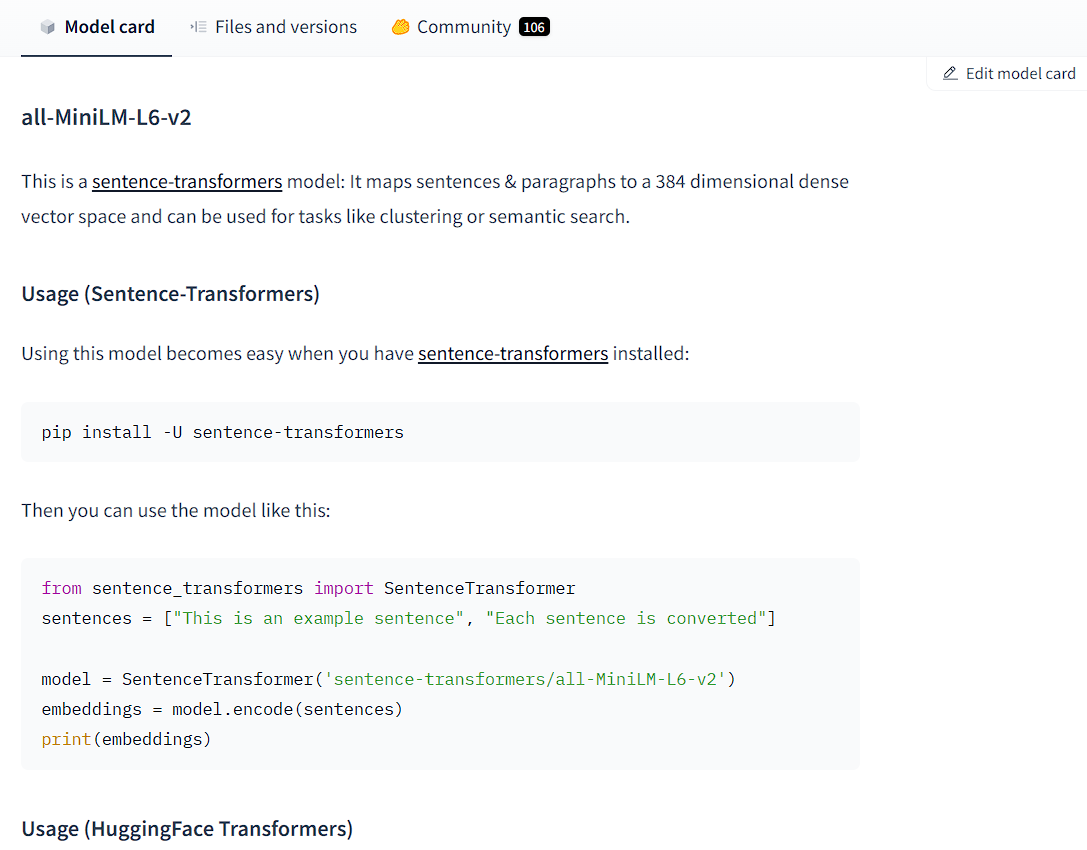
\includegraphics[width=.7\linewidth]{images/model_card.png}
    \caption{Esempio di model card}
    \label{fig1:model_card_completa}
\end{figure}

\subsubsection{Processo di raccolta dati} \label{tirocinio}
Il \textit{data mining}, in questo contesto si rifersce all'attività svolta durante il percorso di tirocinio. Il processo si bassa sulla raccolta, filtraggio e strutturazione degli script Python provenienti da repository pubblici su GitHub, al fine di individuare esempi reali di utilizzo dei modelli di Hugging Face. Questa fase è fondamentale per costruire un dataset affidabile e rappresentativo, propedeutico all'analisi dei pattern di codice e il successivo confronto con le model card ufficiali.
\begin{figure}[htbp]
    \centering
    \includegraphics[width=.9\linewidth]{images/data_collection_new.pdf}
    \caption{Processo di collezione~\cite{CodeXHug}}
    \label{fig:tirocinio}
\end{figure}
L'analisi è iniziata dal dataset di HF ~\cite{ait_hfcommunity_2023} disponibile sotto licenza open-source. Pre-processando e filtrando per specifici task, si è focalizzata l'attenzione su un sotto-insieme di 17,660 PTM.\\
Per identificare i file Python che utilizzano i modelli, si costruiscono delle specifiche query da inviare all'endpoint dell'API di Github~\cite{github_rest}, tramite il client PyGithub~\cite{pygithub}, strutturandole in questo modo:\\
\emph{model\_name} language:\emph{Python}
La funzione di ricerca, eseguita in parallelo, raccoglie, per ogni modello, al massimo 1,000 (limite imposto dalla Rest API) file content in formato utf-8, archiviandoli su una base dati MongoDB \cite{pymongo}. 
Partendo da 17,760 query, 10,335 hanno prodotto zero pagine di risultato per un totale cioè di 7,325 modelli di cui si sono collezionati 453,260 script Python, che costituiscono nell'insieme il punto di partenza dell'approccio adottato in questo lavoro.\\
\begin{table}[htbp]
\small
    \centering    
    \caption{Tags selezionati ed occorrenze dei PTMs}
    \label{tab:tags2}
    \begin{tabular}{|l|l|l|}
    \hline
            Tag & URLs & Contents \\ \hline
            text-generation & 181,153 & 177,913\\ 
            text-to-image & 30,918 & 30,377\\ 
            image-classification & 37,741 & 30,377\\ 
            text-classification & 29,977 & 25,271\\ 
            text2text-generation & 32,743 & 31,541\\ 
            fill-mask & 68,877 & 66,575\\ 
            sentence-similarity & 22,473 & 21,845\\ 
            question-answering & 9,784 & 9,132\\ 
            summarization & 8,057 & 7,820\\ 
            zero-shot-image-classification & 14,132 & 13,900\\ 
            image-to-text & 13,833 & 13,470\\ 
            object-detection & 7,023 & 6,858\\ 
            image-segmentation & 12,002 & 11,725\\ \hline
    \end{tabular}
\end{table}
\subsubsection{LLM} 
\textbf{LLM} (\textit{L}arge \textit{L}anguage \textit{M}odels) sono modelli di linguaggio che rappresentano un'innovazione significativa nell'ambito del \(NLP\) (Natural Language Processing), sono costruiti su reti neurali profonde\cite{di2025use}, in particolare sull'architettura \textit{Transformer}\cite{vaswani2017attention}  che introduce un nuovo paradigma per l'elaborazione del linguaggio naturale.\\ 
L'architettura Transformer è costituita principalmente da due componenti: l'\textbf{encoder}, che elabora il testo in input generando rappresentazioni semantiche, e il \textbf{decoder}, che utilizza tali rappresentazioni per generare l'output. Il processo dell'\textbf{encoder} avviene attraverso una serie di passaggi fondamentali. La prima fase è la tokenizzazione, che converte ogni parola in \textit{token}, ovvero unità fondamentali di elaborazione \cite{huggingface_transformers_tokenizer}. Successivamente, ciascun token viene trasformato in un vettore numerico attraverso la fase di embedding, in cui ogni token viene mappato a una rappresentazione numerica basata su un dizionario del modello \cite{devlin2019bertpretrainingdeepbidirectional}. Poiché i \textit{Transformer} non elaborano il testo in maniera sequenziale, si applica il \textit{positional encoding}, che aggiunge un vettore di posizione per preservare l'ordine delle parole \cite{vaswani2017attention}. A questo punto entra in gioco il \textit{self-attention layer}, che consente a ciascuna parola di "guardare" tutte le altre nel contesto per comprenderne meglio il significato \cite{vaswani2017attention}. Infine, la rappresentazione generata viene ulteriormente elaborata tramite una \textit{feed-forward network (FFN)}, che raffina l'informazione catturando aspetti sintattici e semantici più complessi \cite{vaswani2017attention}.\\
Il \textbf{decoder} utilizza le rappresentazioni generate dall’encoder per produrre il testo di output, seguendo un processo altrettanto complesso. Una delle componenti fondamentali di questa fase è il \textit{masked self-attention layer}, che impedisce al modello di analizzare le parole future durante la generazione del testo, assicurando che la predizione successiva si basi esclusivamente sui token già generati. Il \textit{encoder-decoder attention layer} svolge un ruolo cruciale nell'integrare il contesto dell’input con il testo in generazione: esso assegna un punteggio, in una sorta di mappa, a ciascun token dell'input per determinare quali siano i più rilevanti nel processo di generazione. Infine, le informazioni passano attraverso la feed-forward network, che ne raffina ulteriormente la rappresentazione e le trasmette a una funzione \textit{softmax}. Quest'ultima calcola la probabilità di ogni possibile parola successiva e seleziona quella con il valore più alto, completando così il processo di generazione \cite{vaswani2017attention}.
L'elemento chiave nell'architettura Transformer \textbf{meccanismo dell'attenzione},  presente sia nell'encoder che nel decoder e permette all'LLM di pesare l'importanza di una parola rispetto alle altre. Il calcolo dell'attenzione è espresso nella seguente equazione\cite{vaswani2017attention}:
\begin{equation}
    \text{Attenzione}(Q, K, V) = \text{softmax}\left(\frac{QK^T}{\sqrt{d_k}}\right) V
\end{equation}
dove \textit{Q} (Query) rappresenta la parola che sta cercando informazioni, \textit{K} (Key) è la rappresentazione delle parole potenzialmente rilevanti e \textit{V} (Value) contiene le informazioni effettive associate a ogni parola. Le matrici Q,K,V rappresentano in sostanza tre prospettive diversa di una parola, che vengono calcolate moltiplicando il vettore di embedding per la matrice dei pesi, ovvero i parametri del modello. Infine la softmax,  converte i pesi in probabilità, determinando l'importanza relativa di ciascun token.\\
Nella descrizione delle principali componenti dell'architettura si è parlato indistintamente tra parole e token, ma è fondamentale sottolineare che non sono equivalenti. Un token può corrispondere a un'intera parola, ma in molti casi rappresenta solo una porzione di essa, come prefissi e suffissi, oppure singoli caratteri, specialmente in lingue come il cinese o per simboli speciali. Inoltre, esistono token che rappresentano combinazioni di lettere comuni a più parole, noti come \textit{subword}, che permettono di gestire meglio termini rari e di ottimizzare l'efficienza del modello \cite{mielke2021wordscharactersbriefhistory}.\\
Per trasformare le parole del linguaggio naturale in token, ogni LLM utilizza un particolare tokenizer \cite{huggingface_transformers_tokenizer}, ovvero una componente essenziale che, attraverso un pre-processing, suddivide il testo in unità più piccole e gestibili dal modello. Questo processo include operazioni come rimozione di spazi, normalizzazione e suddivisione in token, garantendo una rappresentazione efficace per la successiva elaborazione.\\
Esistono diverse tecniche di tokenizzazione, una delle principali è la \textit{Subword Tokenization} ovvero una metodologia utilizzata per dividere le parole in parti più piccole, chiamate sotto-unità o subword. Questo aiuta i modelli a gestire sia parole molto comuni che parole rare, senza bisogno di un grande vocabolario. Tra le principali tecniche emerge Byte pair encoding \cite{Sennrich2015NeuralMT} in cui parole comuni (codificate in byte) possono rimanere intere, mentre parole rare vengono suddivise in unità più piccole, consentendo al modello di gestire anche termini sconosciuti attraverso la combinazione di sotto-unità già apprese.\\
È bene precisare che le componenti appena descritte sono la base delle varie implementazioni più complesse degli LLM che in base al task per cui sono stati progettati impiegano varianti dell'architettura, per esempio, ad oggi, tra i modelli di linguaggio più popolari spiccano \textit{BERT} \cite{devlin2019bertpretrainingdeepbidirectional} che utilizza solo l'encoder per compiti di comprensione e classificazione e \textit{GPT}\cite{radford2018improving} solo decoder, ideale per generazione di testo, completamento.\\
Gli LLM sono stati addestrati su un'enorme quantità di dati testuali provenienti da libri, articoli e pagine web acquisendo una forte conoscienza e trovando impiego in numerosi ambiti tra cui la generazione e completamento di codice, assistenza nella documentazione software e traduzioni, sintesi di testuali \cite{di2025use}, partendo sempre da un input testuale.\\
Impartire al modello il compito da compiere non è banale per questo si parla di \textit{prompt engineering} come l'arte del formulare input che guidino l'LLM verso le risposte desiderate. Questo può avvenire secondo queste principali tecniche \cite{di2025use}:
\begin{itemize}
    \item \textit{Few-shot prompting}: inserire nell'input pochi esempi per orientarlo nello svolgimento di un compito, riducendo la necessità di un addestramento approfondito (fine-tuning)
    \item \textit{Zero-shot prompting} al contrario del precedente, affida al modello un compito senza fornire esempi, sfruttandone la sua capacità di generalizzare.
\end{itemize}
Nel prompt, per ottenere risposte accurate e contestualizzate in specifici ambiti, solitamente si assegna un ruolo al modello che deve interpretare. Questo aiuta l'LLM a rispondere in maniera più pertinente al contesto richiesto.\\
Un'importante limitazione di questi modelli di linguaggio sono le \textit{allucinazioni} ovvero un comportanmento del LLM che tende a generare risposte plausibili ma sbagliate o prive di fondamento logico \cite{di2025use}. Ciò può essere dovuto a comprensione errata del contesto oppure alla difficoltà nell’interpretare input ambigui o complessi. Nel contesto di questo esperimento un esempio di allucizione si potrebbe verificare quando l'LLM riceve in input del codice Python e deve estrapolarne pattern d'uso ricorrenti ma genera enera funzioni che non hanno alcun collegamento con il codice originale. Questo può essere dovuto all’incapacità del modello di generalizzare correttamente il compito assegnato. Per mitigare questo problema, si è specificato nel prompt cosa fare quando il modello non è in grado di rispondere. Ad esempio, si può esplicitamente indicare che, in caso di incertezza, bisogna restituire una stringa vuota in modo che la successiva analisi dell'output sia più semplice.\\
Negli ultimi anni, gli \textbf{LLM open-source} hanno acquisito un ruolo sempre più centrale, offrendo un’alternativa accessibile e personalizzabile rispetto ai modelli proprietari. Tra questi spicca \textbf{LLaMA} (Large Language Model Meta AI) \cite{journals/corr/abs-2302-13971}, sviluppato zppunto da Meta.\\
LLaMA è una famiglia di modelli linguistici autoregressivi (ovvero per la generazione del prossimo token si basano su quelli già generati), ottimizzati per garantire prestazioni elevate pur mantenendo un’efficienza computazionale adeguata. La loro archittettura si basa sull'architettura \textit{Decoder-only} ovvero non utilizza l'encoder per generare il testo in output prevedendo sotto-sequenze di token man mano che viene costruito l'output \cite{hou2024large}.\\
Questi modelli sono disponibili in diverse dimensioni (7B, 13B, 33B, 65B parametri in base alla versione) e possono essere utilizzati sia per applicazioni di completamento del testo, sia per attività più avanzate come la capacità di seguire istruzione e generazione di codice \cite{hou2024large}.\\
Quando si utilizza un LLM open-source come LLaMA per generare testo (codice), è possibile personalizzare il comportamento del modello attraverso diversi parametri, che influenzano la creatività, la coerenza e la lunghezza delle risposte. I principali sono:
\begin{itemize}
    \item \textit{max tokens}: imposta il numero massimo di token che il modello può generare in una singola risposta. Valori alti consentono generazioni più lunghe, ma possono consumare rapidamente la finestra di contesto (input e prompt di sistema)
    \item \textit{temperatura}: controlla il livello (intervallo tra 0.0 - 2) di casualità nella generazione del testo\cite{peeperkorn2024temperaturecreativityparameterlarge}. Valori bassi (es. 0.1 - 0.3) rendono le risposte più deterministiche e precise, con meno variazioni tra chiamate successive, mentre valori alti (es. 0.7 - 1.5) aumentano la creatività e diversità, ma allo stesso tempo possono produrre risposte meno coerenti.
    \item \textit{top\_p}: filtra i token meno probabili in base a una soglia cumulativa di probabilità. Valori bassi (es. 0.3 - 0.5) rendono i risultati più conservativi, facendo sì che il modello scelga solo tra i token più probabili, mentre valori più alti (es. 0.9 - 1.0) permettono una maggiore diversità nella generazione del testo \cite{Ruman2024}.
    \item \textit{top\_k}: limita la scelta del modello ai primi
    k (naturale) token più probabili in ogni passo di generazione. Un valore basso riduce la casualità, poiché il modello considera solo un insieme ristretto di opzioni, mentre un valore più alto aumenta la varietà delle risposte, ma può introdurre più casualità e incoerenza \cite{Ruman2024}. Se il parametro non è impostato l'LLM considera tutti i token disponibili in base alle loro probabilità.
\end{itemize}

\subsubsection{Clustering}


\subsection{Motivazione} \label{motivation}
Oltre alla misurazione di quanto la generazione automatica di codice, che rappresenti l'uso del modello in contesti reali, sia simile a quella ufficiale presente sulla piattaforma Hugging Face, i risultati condotti dall'esperimento possono essere interpreti anche come una fonte di arricchimento, soprattutto nelle model card in cui non ci sono esempi di codice.

ESEMPIO DI CARD "microsoft/git-large" senza codice (motivazione)

\section{Lavori correlati}
In questa sezione vengono presentati i principali studi e strumenti esistenti che affrontano tematiche affini a quelle trattate in questo esperimento. L'analisi della letteratura permette di contestualizzare il lavoro svolto, evidenziando le soluzioni già proposte, i loro punti di forza e le eventuali limitazioni.

\subsection{Sistemi tradizionali per riuso di codice:}
Il riuso del codice è un aspetto centrale nello sviluppo software, in quanto consente di ridurre il tempo di implementazione, migliorare la qualità del software e facilitare la mantenibilità. Tuttavia, individuare frammenti di codice riutilizzabili e integrarli in nuovi progetti rappresenta una sfida complessa.\\
Un esempio significativo di sistema che si colloca in questo contesto è \textbf{FOCUS}\cite{nguyen2021recommending}. Si tratta di un sistema di raccomandazione di chiamate API e snippet di codice basato su un approccio di collaborative filtering. Il sistema analizza grandi quantità di codice open-source per identificare pattern di utilizzo delle API e suggerire frammenti di codice pertinenti agli sviluppatori. Questo approccio permette di superare le limitazioni delle fonti tradizionali, come Stack Overflow o documentazioni ufficiali, che spesso forniscono esempi incompleti o generici.\\
Il funzionamento del sistema si basa su diverse fasi:
\begin{itemize}
    \item L’analisi di repository open-source, da cui vengono estratti pattern di utilizzo delle API per lo sviluppo di applicazioni mobili
    \item Un motore di raccomandazione che utilizza metriche di similarità per suggerire chiamate API pertinenti al contesto di sviluppo
    \item La possibilità di fornire snippet di codice interi, riducendo lo sforzo manuale degli sviluppatori
\end{itemize}
L’efficacia del sistema è stata dimostrata su un dataset di 2.600 applicazioni Android, mostrando un miglioramento rispetto ad altri sistemi di raccomandazione di API come UP-Miner e PAM. Inolte, è stato condotto un esperimento simulando lo sviluppo di codice e misurando quanto efficacemente FOCUS riusciva a suggerire frammenti di codice mancanti nelle applicazioni Android analizzate.\\
Nel complesso il sistema \textit{FOCUS} presenta diverse analogie con l'approccio proposto in questo esperimento. In particolare:
\begin{itemize}
    \item \textit{Analisi del codice open-source}: anche in questo caso è stato adotatto un processo di data-mining però focalizzato a raccogliere e analizzare oltre 140.000 script Python. per identificare pattern d’uso reali dei modelli di Hugging Face, mentre FOCUS si concentra su progetti software per estrarre pattern di chiamate API.
    \item \textit{Identifazione pattern}: FOCUS utilizza collaborative filtering per suggerire API pertinenti, mentre in questo espresimento si clusterizza e sintetizzano snippet di codice ricorrenti per derivare best practices di utilizzo dei modelli; in entrambi i casi i risultati vengono valutati attraverso metriche di similarità
    \item \textit{Supporto agli sviluppatori}: entrambi i sistemi hanno come obbiettivo principale quello di aiutare i programmatori nello sviluppo software, riducendo gli sforzi.
\end{itemize}

\subsection{Generazione di codice tramite LLMs:}
L’uso dei modelli di linguaggio di grandi dimensioni ha rivoluzionato il modo in cui gli sviluppatori scrivono software. Lo studio\cite{hou2024large} presenta un'analisi sistematica della letteratura scientifica applicata all'ingegneria dell'software, analizzando oltre 395 articoli pubblicati tra il 2017 e il 2024.\\
I principali utilizzi degli LLMs nella generazione di codice includono:
\begin{itemize}
    \item \textit{Completamento del codice}: strumenti come Codex (da cui deriva GitHub Copilot) suggeriscono frammenti di codice mentre l’utente scrive
    \item \textit{Generazione automatica di funzioni}: i modelli possono produrre intere funzioni sulla base di specifiche in linguaggio naturale
    \item \textit{Traduzione tra linguaggi di programmazione}: conversione automatica del codice tra diversi linguaggi.
\end{itemize}
L'analisi effettuata si collega direttamente a questo lavoro, perché si sfrutta un LLM per sintetizzare pattern di codice rappresentativi reali basandosi sugli snippet estratti da progetti open-source, un approccio simile Codex e AlphaCode, ma con l'obbietivo di automatizzare e migliorare la documentazione dei PTM di Hugging Face.\\
Inoltre, l'utilizzo di metriche di similità come \textit{CodeBLEU} sono fondamentali per l'accuratezza e la valutazione del codice generato dagli LLMs.

\section{Approccio}
Immagine e spiegazione legenda\\
Nell'immagine (ref) è raffigurata la pipeline del lavoro partendo dal dataset prodotto nella sezione \ref{tirocinio}, fino alla generazione di pattern riccorenti tramite LLM. La legenda indica per ogni numero presente a quale tipo di dato ci si sta riferendo.\\
\subsection{Filtro modelli popolari}
\begin{figure}[h]
    \centering
    \begin{minipage}{0.45\textwidth}
        \centering
        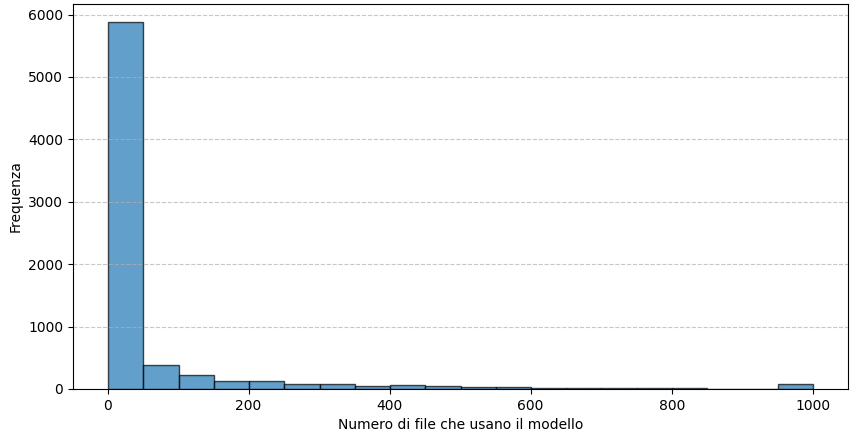
\includegraphics[width=\linewidth]{images/approccio1.png}
        \caption{Distribuzione dei file}
        \label{fig:distribuzione_file1}
    \end{minipage}
    \hfill
    \begin{minipage}{0.45\textwidth}
        \centering
        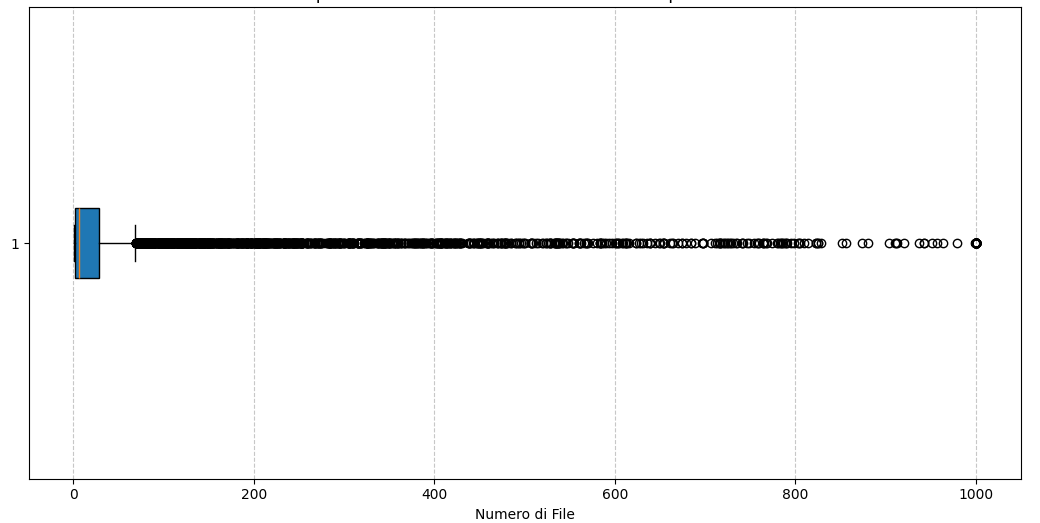
\includegraphics[width=\linewidth]{images/approccio2.png}
        \caption{Analisi outlier}
        \label{fig:outlier_file1}
    \end{minipage}
\end{figure}
Il database prodotto nella parte di tirocinio contiene per 7,325 PTM un totale di 453,260 file sorgenti Python. La distribuzione \ref{fig:distribuzione_file1} dei dati è fortemente asimmetrica, presentando un'elevata concentrazione di modelli con un numero molto basso di codici mentre solo un ristretto numero di PTM è utilizzato in una quantità significatamente maggiore di file.\\
In particolare, la distribuzione segue un andamento tipico delle distribuzioni \textit{long tail} che si manifesta con una forte asimmetria positiva (right-skewed distribution) evidenziando che la maggior parte dei modelli è utilizzata in pochissimi file mentre modelli altamente popolari sono in una frequenza molto minore.\\
\begin{table}[h]
    \centering
    \begin{tabular}{|l|c|}
        \hline
        \textbf{Metrica} & \textbf{Valore} \\
        \hline
        Media & 63.99 \\
        Mediana & 6.00 \\
        Deviazione Standard & 162.54 \\
        Skewness & 3.86 \\
        Kurtosis & 16.09 \\
        \hline
    \end{tabular}
    \caption{Metriche statistiche per il numero di file per modello}
    \label{tab:metriche_file_modello1}
\end{table}\\
Infatti dalle informazioni statiche \ref{tab:metriche_file_modello1}, la mediana è molto inferiore alla media e la deviazione standard elevata conferma l'alta variabilità tra i modelli. Inoltre, la notevole skewness evidenzia che la distribuzione è sbilanciata a destra, con alcuni modelli molto più utilizzati rispetto alla maggioranza. Infine la curtosi indica la presenza di numerosi \textit{outlier}, cioè modelli con un utilizzo estremamente superiore rispetto alla norma.\\
Per evitare possibili distorsioni negli esperimenti successivi dell'approccio, si è deciso quindi di selezionare un sottoinsieme di PTM aventi un numero di file arbitrariamente maggiore di 100 formato da 1,064 modelli per un totale complessivo di 393,484 script.\\
\begin{figure}[h]
    \centering
    \begin{minipage}{0.45\textwidth}
        \centering
        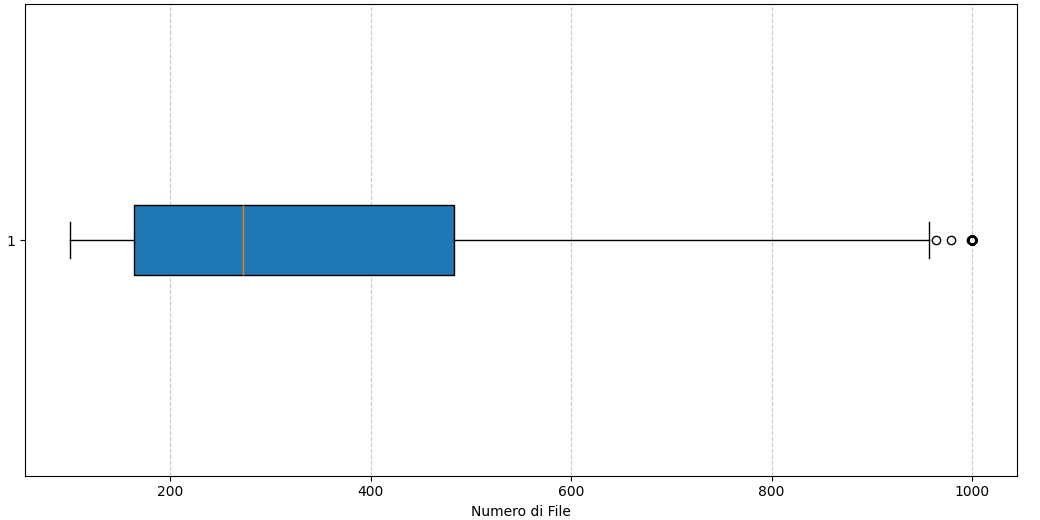
\includegraphics[width=\linewidth]{images/approccio3.png}
        \caption{Distribuzione dei file filtrati}
        \label{fig:distribuzione_file2}
    \end{minipage}
    \hfill
    \begin{minipage}{0.45\textwidth}
        \centering
        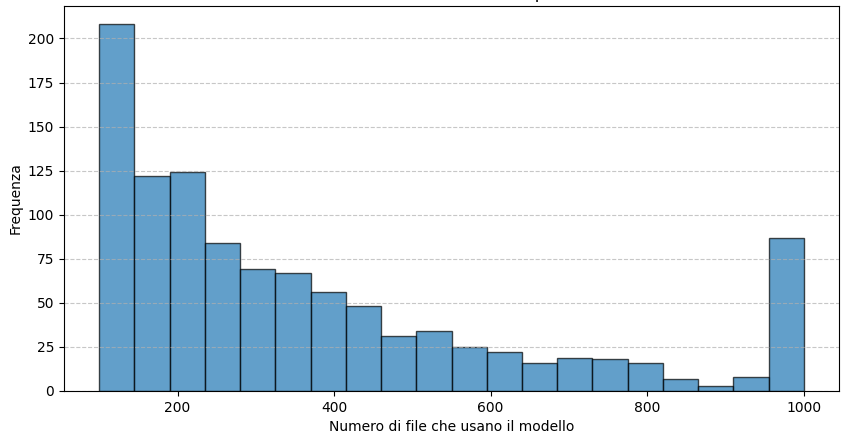
\includegraphics[width=\linewidth]{images/approccio4.png}
        \caption{Analisi outlier post filtro}
        \label{fig:outlier_file2}
    \end{minipage}
\end{figure}
Dopo aver applicato il filtro selezionando solo i modelli con almeno 100 file associati, la distribuzione \ref{fig:distribuzione_file2} mostra caratteristiche significativamente diverse rispetto a quella originale.\\
\begin{table}[h]
    \centering
    \begin{tabular}{|l|c|}
        \hline
        \textbf{Metrica} & \textbf{Valore} \\
        \hline
        Media & 369.82 \\
        Mediana & 6.00 \\
        Deviazione Standard & 265.65 \\
        Skewness & 1.17 \\
        Kurtosis & 0.31 \\
        \hline
    \end{tabular}
    \caption{Metriche per il numero di file per modello post filtro}
    \label{tab:metriche_file_modello2}
\end{table}\\
Inoltre, dalle nuove metriche \ref{tab:metriche_file_modello2} la media è aumentata da 63.99 a 369.82, e la mediana è passata da 6 a 272.50, indicando che ora ci si sta concentrando solo sui modelli più popolari.La deviazione standard di 265.65 mostra ancora una notevole variabilità nel numero di file per modello, sebbene ridotta rispetto alla distribuzione completa. L’asimmetria (skewness) si è ridotta drasticamente da 3.86 a 1.17, suggerendo che la distribuzione è ora meno sbilanciata a destra. Inoltre, la curtosi è passata da 16.09 a 0.31, indicando una distribuzione più piatta con meno outlier estremi.\\
Questo filtraggio ha quindi permesso di eliminare la gran parte dei modelli con utilizzo marginale, garantendo un'analisi più bilanciata dei modelli più diffusi.
Oltre a ridurre le distorsioni dovute alla scarsità di dati, la selezione si è basata anche sul cercare di includere i modelli più popolari e ampiamente utilizzati sulla piattaforma, al fine di concentrarsi sui modelli effettivamente reliventi per la community.\\
I nomi dei modelli selezionati sono stati salvati in un file JSON in modo da essere facilmente accessibili e utilizzabili nelle fasi successive.


\subsection{Filtro dei codici sorgenti per lunghezza}
(IMMAGINE)\\
Per migliorare l'efficienza della successiva ricerca delle porzioni più rilevanti dei file si è implementato un processo di selezione degli script, precedentemente filtrati, basato sulla lunghezza degli stessi.\\
L'idea di base è che alcuni codici troppo brevi potrebbero non contenere informazioni significative sull'utilizzo di un particolare modello e allo stesso modo codici troppo lunghi potrebbero includere porzioni non pertinenti come ad esempio descrizioni e lunghi commenti.\\
Il processo di filtraggio si basa nel considerare solo gli script che hanno una lunghezza in termini di linee di codice comprese nell'intervallo interquantile (IQR), utilizzando la mediana come valore centrale. In particolare, l'IQR è una misura statistica della dispersione dei dati così definita:
\begin{equation}
    IQR = Q3 - Q1
\end{equation}
dove Q1 (primo quartile) indica il valore sotto il quale si trova il 25\% dei file più corti, mentre Q3 (terzo quartile) il valore sotto il quale si trova il 75\% dei file. Quindi, il risultato rappresenta l'ampiezza della fascia centrale della distribuzione cioè pari al 50\% dei dati.\\
Nella pratica la mediana e l'IQR vengono così impiegati nel calcolo nell'intervallo di selezione:
\begin{equation}
    min\_length =max(mediana-0.25*IQR,1)
\end{equation}
\begin{equation}
    max\_length =mediana+0.25*IQR
\end{equation}
dove il fatore 0.25 permette di restringere l'intervallo intorno alla mediana senza essere troppo rigido.\\
Di conseguenza, questo range permette di selezione i file in base alla loro lunghezza attraverso una misura più robusta della media, concentrandosi su insieme più omogeneoe ed escludendo la presenza di eventuali outlier.\\
Per ottimizzare il tempo di elaborazione dei vari calcoli, il processo viene eseguito in parallelo utilizzando il multithreading perché si tratta prevalentemente di operazioni di lettura e scrittura su disco (I/O bound) in quanto calcolo matematico è piuttosto semplice. Nel dettaglio ogni thread lavora su un sottoinsieme di file riducendo l'attesa rispetto ad un'elaborazione sequenziale. Inoltre, l'uso di un \textit{ThreadPoolExecutor}\cite{python-concurrent-futures} garantisce una gestione automatica delle risorse, bilanciando il carico di lavoro tra i thread attivi.\\
I path dei file la cui lunghezza rientra nell'intervallo dinamico calcolato, vengono salvati in un file JSON cosicchè da avere un riferimento diretto all'archivio locale del dataset.

\subsection{Ricerca dei migliori \textit{code snippet}}
(IMMAGINE)\\
L'LLM preso in considerazione per questo esperimento ha una finestra di contesto molto limitata, ovvero non riesce a gestire per ogni chiamata più di un certo numero di token in input e in output.\\
L'ipotetico approccio di far valutare al modello direttamente interi script Python, senza un pre-processing, potrebbe essere molto restrittivo in termini di possibili pattern di codice da scoprire, nonché inefficiente perché gli stessi script potrebbero non avere un interessante senso semantico. Per esempio, alcuni file, si potrebbere limitare soltanto a menzionare il modello in esame con commenti e descrizioni senza poi impiegarlo realmente.\\
Per affrontare queste problematiche, si è deciso di analizzare in maniera automatica ogni singolo file filtrato dalla sezione precedente, con l'obiettivo di estrapolarne una porzione che fosse la più rappresentativa e rilevante possibile in termini di utilizzo del modello, provando a non considerare per esempio sezioni di debugging o funzioni di utility non significative. Il processo di estrazione è basato sulla ricerca di parole chiavi legate fortemente all'addestramento, tokenizzazione e inferenza standard dei PTM disponibili su HF. In particolare, l'implementazione è suddivisa in 5 fasi:\\
\subsubsection{Analisi della struttura del codice}
Per ogni file Python risultante dal calcolo della mediana viene utilizzo un parser per \textbf{l'Abstract Syntax Tree (AST)} \cite{python_ast}, ovvero una rappresentazione sintattica strutturata del codice sorgente. Ciò permettere di iterare sui nodi dell'albero per identificare importazioni di librerie e definizioni di funzioni (incluso il loro corpo) che contengono (match) almeno una delle keyword definite. \\
La ricerca della corrispondenza viene effettuata a livello di linea: per fornire un contesto più ampio e facilitare la comprensione dello snippet estratto, vengono aggiunte due (arbitrariamente) righe di contesto sia prima che dopo la porzione individuata.\\
Tuttavia, l’analisi AST potrebbe fallire in presenza di errori sintattici nel codice sorgente come parentesi mancanti, indentazioni errate, stringhe non chiuse correttamente. In questi casi l'errore viene solo segnalato a schermo e il file scartato dal processo successivo.\\
\textbf{KEYWORD}:
\lstset{basicstyle=\ttfamily, columns=flexible}
\begin{lstlisting}
import, from, transformers, huggingface, 
AutoModel, AutoTokenizer, AutoConfig, pipeline,
train, fit, fine_tune, finetune,
token, tokenizer, encode, decode,
predict, inference, generate, metric,
sklearn, scikit-learn
\end{lstlisting}
    
\subsubsection{Raggruppamento delle informazioni}: dopo l'individuazione delle diverse porzioni pertinenti può accadere che più frammenti siano vicini tra loro condividendo alcune righe di codice. Per evitare ripetizioni ridondanti, questi frammenti vengono unificati mediante la fusione degli intervalli di righe sovrapposti, garantendo che snippet contigui non vengano considerati separatamente. 

\subsubsection{Ricerca del miglior snippet}
L'analisi sintattica e il successivo raggruppamento restituiscono, per ogni file, un insieme di snippet contenenti almeno una corrispondenza con le keyword definite. Tuttavia, per scegliere il migliore tra i candidati è necessario considerare anche il significato semantico del codice.\\
Per raggiungere questo obiettivo, si è utilizzato l'algoritmo \textbf{K-means} implementato con la libreria \textit{scikit-learn}\cite{scikit-learn} che opera su una rappresentanzione numerica delle informazioni. Poiché gli snippet sono inizialmente sotto forma di stringhe, è stato adottato un modello di embeddings (\cite{all-MiniLM-L6-v2}) fornito da Hugging Face tramite la libreria \textit{sentence\_transformers}. Questo modello, basato sull’architettura \textit{Transformer} e in particolare in una versione ridotta di \textit{BERT}, converte ogni snippet in un vettore numerico di 384 dimensioni attraverso una pipeline di tokenizzazione, calcolo dell’attenzione e infine generazione dell’embedding tramite mean pooling (media pesata di tutti gli embedding dei token). Nonostante i modelli della libreria \textit{sentence\_transformers} siano principalmente progettati per il linguaggio naturale riescono comunque a catturare molte informazioni sintattiche e semantiche nei frammenti di codice soprattutto se l'obbiettivo è selezionare gli snippet rappresentativi e non necessariamente eseguire un'analisi profonda delle operazioni a basso livello di codice. Inoltre, è particolarmente utile quando sono presenti commenti in linguaggio naturale che spiegano determinare strutture nel codice.\\ 
Si è deciso di adottare questo tipo di embedder anche per un trade-off tra prestazioni e leggerezza, perché utilizzando ad esempio \textit{CodeBERT}\cite{feng2020codebertpretrainedmodelprogramming} i tempi di inferenza e utilizzo della memoria per centinaia di migliaia di file sarebbero stati sicuramente più alti. 
Gli embeddings ottenuti vengono passati al \textit{K-means} che ha il compito di assegnarli in $k$ cluster. Il valore di $k$ viene scelto empiricamente come il minimo tra un valore fisso pari a 3 e la lunghezza della lista degli snippet, in modo da adattarsi dinamicamente al numero di candidati disponibili.\\
L'algortimo K-means funziona seguendo i seguenti passaggi:
\begin{itemize}
    \item \textit{Inizializzazione dei centroidi}: i centroidi, ovvero i punti che rappresentano il centro di ciascun cluster, vengono inizializzati in modo da essere il più distanti possibile tra loro partendo dagli embegginds di input.
    \item \textit{Assegnazione dei punti ai cluster}: ogni embedding viene assegnato al cluster il cui centroide è più vicino in termini di distanza euclidea. Formalmente la distanza tra un embedding $x$ e un centroide $c$ è calcolata:
    \begin{equation}
        d(x, c) = \sqrt{\sum_{i=1}^{384} (x_i - c_i)^2}
    \end{equation}
    \item \textit{Ricalcolo dei centroidi}: una volta assegnati tutti i punti, per ogni cluster si calcola un nuovo centroide come media aritmetica (punto o vettore medio) degli embeddings appartenenti al cluster. Se $C_{j}$ è l'insieme dei punti del cluster $j$ allora il nuovo cluster $c_{j}$ è definito:
    \begin{equation}
        c_j = \frac{1}{|C_j|} \sum_{x \in C_j} x
    \end{equation}
    \item \textit{Iterazione fino alla convergenza}: I passaggi di assegnazione e ricalcolo dei centroidi vengono ripetuti fino a quando i centroidi non si stabilizzano ovvero non cambiano significativamente tra due iterazioni consecutive, segnando che l'algoritmo sta convergendo
\end{itemize}
Una volta raggiunta la convergenza, per ogni cluster si seleziona lo snippet il cui embedding è più vicino al rispettivo centroide. Tale snippet viene considerato il più rappresentativo del gruppo, poiché riassume al meglio le caratteristiche semantiche condivise dagli altri elementi del cluster.\\

\subsubsection{Elaborazione parallela}
Per ottimizzare i tempi di esecuzione, in presenza di un elevato numero di file da elaborare, anche questa sezione, il processo è stato parallelizzato tramite l’utilizzo del \textit{multithreading}. Ciascun thread si occupa di elaborare in modo indipendente un file, estraendo gli snippet, calcolando gli embeddings e applicando l’algoritmo di clustering. Questo approccio consente di ridurre significatamene i tempi complessivi di esecuzione.

\subsubsection{Salvataggio informazioni}
L'insieme degli snippet selezionati da ogni cluster vengono infine salvati in un file JSON per facilitarne la consultazione e l’utilizzo nella successiva fase di analisi, secondo la seguente struttura:\\\\\\
\begin{lstlisting}[language=json, caption={Esempio di struttura JSON dei migliori snippet selezionati}, label={lst:json-example}]
{
  "bert-base-uncased": {
    "path/to/file1.py": [
      "import transformers\n\nmodel = AutoModel.from_pretrained('bert-base-uncased')",
      "tokenizer = AutoTokenizer.from_pretrained('bert-base-uncased')\ninputs = tokenizer('Hello world', return_tensors='pt')"
    ],
    "path/to/file2.py": [
      "pipeline = transformers.pipeline('sentiment-analysis')\nresult = pipeline('I love coding!')"
    ]
  },
  "roberta-base": {
    "path/to/file3.py": [
      "import transformers\nmodel = AutoModel.from_pretrained('roberta-base')"
    ]
  }
}
\end{lstlisting}
Questa pipeline consente di selezionare automaticamente, per ciascun file, le porzioni di codice più rappresentative in termini di utilizzo dei modelli di Hugging Face, riducendo la quantità di codice irrilevante da fornire successivamente all'LLM.


\subsection{Utilizzo dell'LLM}
(IMMAGINE)\\
Nel contesto di questo esperimento, è stato sfruttuano un particolare LLM opensource per analizzare gli snippet di codice Python estratti precedentemente, al fine di indiduare schemi comuni nell'utilizzo dei PTM tramite le principali librerie della piattaforma di Hugging Face.
L'obiettivo è di isolare pattern significativi senza dover eseguire un'analisi manuale per ciascun modello esaminato, riducendo tempi e sforzi operativi.
\subsubsection{Flusso operativo}
L'idea di base è fornire, per ogni modello in esame, il maggior numero possibile di snippet, cercando di massimizzare l’utilizzo dei token di input disponibili per l’LLM. Per garantire coerenza e confrontabilità tra le varie chiamate, viene utilizzato un \textit{prompt} fisso per tutti i modelli. \\
Il prompt ha come unico scopo di istruire il modello a individuare eclusivamente pattern di codice, come:
\begin{itemize}
    \item importazioni comuni
    \item definizioni di funzione
    \item strutture tipiche di utilizzo dei modelli PTM
\end{itemize}
La tecnica utilizza nella costruzione è \textit{zero-shot prompting} perché non si menzionano esempi nella stringa, puntanto sulla capicità del modello di generalizzare nelle risposte.
\begin{lstlisting}[]
system_prompt = (
"You are an AI assistant specialized in Python.
I will provide you with a series of code snippets extracted from various Python files.
Note that these snippets might not form a coherent or complete code module when combined together.
Your task is to analyze these snippets and extract recurring code patterns, such as function definitions (using 'def'), common imports, and other typical structures found in Python code.
Focus solely on identifying and returning the common patterns in the context of the model {snippet_model}.
Return ONLY the code snippets.
DO NOT include only the common imports.
Do NOT include any explanations, descriptions, or metadata.
Do NOT generate any summaries, bullet points, markdown formatting, or additional text.
If you are unable to find any relevant patterns, please return an empty string."
)    
\end{lstlisting}
Si può notare come nel prompt venga specificato un ruolo di assistente Python per cercare di contestualizzare al meglio le risposte. Inoltre, si definiscono dei vincoli nella generazione dell'output per evitare che contengano testo potenzialmente non necessario. Queste ipotetiche descrizioni superflue potrebbero alterare la fase di validazione, perché si confronterebbe del linguaggio naturale con codice Python alternando i risultati delle metriche.
Per la scelta delle porzioni di codice da inviare al modello, viene effettuato un primo filtro: tramite espressioni regolari vengono selezionati solo gli snippet contenenti almeno il nome del modello e la keyword "def". Questo controllo garantische che gli snippet siano pertinenti con il modello in esame e che venga inclusa almeno una definizione di funzione, rendendo il codice rilevante per l'identificazione di pattern funzionali.\\
Una volta selezionati gli snippet l'input per l'LLM viene costruito in maniera incrementale:
\begin{itemize}
    \item gli snippet vengono aggiunti uno alla volta alla stringa da inviare
    \item dopo ogni aggiunta, si calcola il numero di token complessivi utilizzando il tokenizer del modello
    \item il processo continua finché non si raggiunge il limite massimo di token previsto
\end{itemize}
Il numero massimo di token disponibili per l’input è calcolato come segue:
\begin{equation}
    allowed\_input\_tokens = max\_total\_tokens - system\_tokens - reserved\_output\_tokens
\end{equation}
dove
\begin{itemize}
    \item \textit{allowed\_input\_tokens}: numero di token disponibili, che aumenta con il crescere degli snippet selezionati
    \item \textit{max\_total\_tokens}: limite imposto dal modello pari a 4096 token
    \item \textit{system\_tokens}: numero token occupati dal prompt di sistema, considerabile costante a eccezione della variazione dovuta al nome del modello
    \item \textit{reserved\_output\_tokens} termine costante pari a 400,  riservati per l’output dell’LLM
\end{itemize}
Questo approccio garantisce l'utilizzo ottimale della finestra di contesto del modello, permettendo di massimizzare le informazioni fornite rispettando i limiti imposti.\\
Per ottenere risposte più accurate, coerenti e meno soggette a variazioni casuali, nella chiamata all'LLM viene impostata una \textit{temperatura} pari a 0.2. L'obiettivo è l’individuazione precisa di pattern di codice piuttosto che una generazione creativa, quindi l'uso di una bassa temperatura riduce la variabilità tra le risposte e minimizza il rischio di ottenere output fuorvianti o allucinazioni. Inoltre il parametro\textit{top\_p} è impostato a 1.0, il che significa che la selezione dei token successivi avviene considerando l'intera distribuzione di probabilità prodotta dal modello senza introdurre un bias artificiale che potrebbe penalizzare alternative comunque valide. A differenza di valori più bassi di top\_p, che avrebbero ristretto la scelta ai token con le probabilità più alte fino a raggiungere la soglia cumulativa, consentendo quindi di sfruttare appieno il potenziale del modello senza escludere a priori opzioni meno probabili che potrebbero comunque risultare rilevanti.\\
La richiesta all'LLM avviene tramite la seguente chiamata:
\begin{lstlisting}
        completion = client.chat.completions.create(
            model=llm_model,
            messages=messages,
            max_tokens=reserved_output_tokens,
            temperature=0.2, 
            top_p=1.0
        )
\end{lstlisting}
Il parametro \textit{messages} contiene il contesto della conversazione ovvero il prompt, precendemente definito, associato al ruolo di sistema che l'LLM deve assumere, seguito dal contenuto vero e proprio costruito iterativamente sull'insieme di snippet di codice.\\
Per ogni risposta ricevuta dall'LLM, l'algoritmo implementa una semplice logica di validazione per verificarne la pertinenza e la qualità. In particolare, In particolare, il sistema verifica che l'output soddisfi due criteri fondamentali:
\begin{itemize}
    \item Contenga il nome del modello analizzato, confermando che il contesto richiesto sia stato effettivamente considerato
    \item Includa almeno le keyword "import" e "def", per garantire la presenza di sezioni di codice Python, essenziali nell'analisi dei pattern
\end{itemize}
Se l'output non soddisfa uno o entrambi questi criteri, il sistema effettua automaticamente fino a due nuovi tentativi con lo stesso input, ripetendo la validazione dopo ogni risposta. Ripetere la chiamata permette di provare a moderare la variabilità nelle risposte, aumentando la probabilità di ottenere un output valido e pertinente.\\ 
Nel caso in cui, anche dopo tre tentativi complessivi, la risposta non risulti conforme ai criteri stabiliti, viene comunque considerato valido l'ultimo output generato. Questa scelta evita cicli infiniti e garantisce che almeno un risultato venga prodotto per la successiva fase di testing. \\
Può comunque accadere che l'output dell'LLM sia vuoto, perché se la fase di scelta degli snippet da inviare non produce corrispondenza, l'intero input è vuoto e quindi il modello risponde di conseguenza con una stringa nulla.\\
Infine, L’output viene salvato in un file JSON avente la seguente struttura: 
\begin{lstlisting}[language=json, caption={Esempio di struttura JSON nella risposta dell'LLM}, label={lst:json-example}]
{
    "nome_modello_1": {
        "system_prompt": "Testo del prompt contenente il nome del modello 1",
        "user_input": [
            "Snippet di codice selezionato casualmente 1",
            "Snippet di codice selezionato casualmente 2"
        ],
        "llm_output": "Risultato generato dall'LLM in risposta all'input fornito",
        "input_tokens": 1234,
        "reserved_output_tokens": 400,
        "attempts": 1,
        "temperature": 0.2
    },
    "nome_modello_2": {
        "system_prompt": "Testo del prompt Testo del prompt contenente il nome del modello 2",
        "user_input": [
            "Snippet di codice selezionato casualmente 1",
            "Snippet di codice selezionato casualmente 2"
        ],
        "llm_output": "Risultato generato dall'LLM in risposta all'input fornito",
        "input_tokens": 1456,
        "reserved_output_tokens": 400,
        "attempts": 2,
        "temperature": 0.2
    }
}
\end{lstlisting}
In sintesi, questo approccio consente di massimizzare l’efficacia delle chiamate all’LLM, garantendo che:
\begin{itemize}
    \item gli snippet inviati siano pertinenti e rappresentativi
    \item le risposte contengano informazioni utili e coerenti con l’obiettivo dell’esperimento
    \item venga rispettato il limite di token imposto dal modello
\end{itemize}

\subsubsection{Esempio di card generata}

\section{Validazione e risultati}
(IMMAGINE)\\
\subsection{Scelta LLM e modalità} \label{scelta LLM}
L'LLM adoperato per l'intero processo è \textbf{meta-llama/Llama-3.2-3B-Instruct}, sviluppato appunto da meta e appartenente alla collezione \textit{Llama 3.2}. Questa versione è progettata per essere utilizzata in compiti di tipo "instruct" (ovvero guidata da prompt specifici) e supporta l’elaborazione di un massimo di 4.096 token per ogni chiamata, suddivisi tra input e output.  
Per accedere al modello, è stato utilizzato il servizio \textit{Hugging Face Inference API} un sistema consente di inviare richieste autenticate tramite token personale e ottenere risposte direttamente dai modelli open-source disponibili .\\
Questo approccio offre diversi vantaggi:
\begin{itemize}
    \item Eliminazione vincoli hardware: eseguire un LLM di queste dimensioni su una macchina locale richiede un potenza di calcolo media-alta con la necessità di disporre di GPU dedicata con ampie quantità di VRAM
    \item Semplicità d'uso e deployment immediato: non è neccassario installare localmente il modello nè configurare l'ambiente perché l'API fornisce un'interfaccia semplice per inviare e ricevere risposte facilmente integrabile nel proprio sistema
    \item Ottimizzazione dei tempi di risposta: la richiesta remota comporta, ovviamente, una latenza di rete ma il tempo complessivo rimane sempre inferiore rispetto al gestire locale il modello (con un hardware limitato)
\end{itemize}
\subsection{Valutazione}
L'obbietivo principale è valutare l'efficacia e la qualità delle model card generate automaticamente dall'LLM rispetto a quelle ufficiali presenti sulla piattaforma di Hugging Face.  Questo confronto ha lo scopo di misurare quanto i codici creati siano pertinenti e, soprattutto, utili per gli sviluppatori finali, che si potranno affidare a questi esempi per comprendere come utilizzare correttamente i PTM.

\subsubsection{Costruzione dataset di test}
Nonostante nel dump \cite{ait_hfcommunity_2023}  ci fosse la feature "card data", cioè le informazioni riguardanti la model card di ogni PTM, non erano presenti gli snippet di codice Python che mostrano l'utilizzo del modello specifico in un esempio di applicazione.\\  
Quindi, per ottenere queste sezioni della card di HF, si è sviluppato un semplice script che utilizza la libreria \textit{BeautifulSoup}\cite{Richardson_Beautiful_Soup} per effettuare web scarping delle pagine HTML dei PTM popolari selezioni per l'esperimento. Ad ogni iterazione si ricerca il tag \textit{\textless code\textgreater} e quando avviene la corrispondenza si controlla che il risultato sia effettivamente appartenente al linguaggio Python, quindi semplicemente verificando che nella stringa siano presenti le keyword "import", "from" e "def".\\
Si noti che per ogni PTM analizzato lo scraper potrebbe trovare anche più di uno snippet Python, perché nella stessa model card potrebbe venir illustrate diverse pipeline di utilizzo: dall'importazione con diverse librerie (per esempio \textit{transformers} e \textit{sentence\_transformers}) fino a metodi di encoding tramite embeddings.\\
Il dataset è strutturato secondo il seguente formato JSON:\\
\\
Dall'analisi effettuata il risultato è di 751 modelli che nelle proprie model card contengano almeno uno snippet di codice Python rispetto ai 1064 di partenza. La differenza è composta quindi da PTM che nonostante siano mediamente popolari sull'utilizzo pratico in progetti open-source abbiano una documentazione probabilmente non completa ed efficace agli sviluppatori; ciò motiva maggiormente lo scopo generale di questo studio.

\subsubsection{Metriche}
Dopo aver raccolto le card ufficiali, si è proceduti nel valutare quanto fossero simili a quelle generate dall'LLM. Sono state impiegate tre metriche di confronto che valutano la somiglianza a livello lessicale, semantico e strutturale del codice:
\begin{itemize}
    \item \textbf{METEOR} (Metric for Evaluation of Translation with Explicit ORdering) \cite{banerjee2005meteor} è progettata principalmente per la valuzione di traduzioni automatiche confrontando le parole secondo un matching flessibile ovvero la corrispondenza si basa su sinonimi, stemmatura e ordine con cui compaiono. Questa flessibilità permette di catturare non solo l'aspetto sintattico ma anche una parziale sensibilità semantica perché, per esempio, la definizione di una funzione potrebbe essere scritta in due modi diversi ma rappresentare lo stesso significato.\\
    Il calcolo della metriche è il seguente:
    \begin{equation}
        \text{METEOR} = (1 - \text{penalty}) \cdot F_{\text{mean}}
    \end{equation}
    dove:
    \begin{equation} \label{penality_meteor}
        \text{penalty} = \gamma \left( \frac{\text{numero di chunk}}{\text{numero di parole corrispondenti}} \right)^\beta
    \end{equation}
    \begin{equation} \label{media_meteor}
        F_{\text{mean}} = \frac{10 \cdot P \cdot R}{9P + R}
    \end{equation}
    \begin{itemize}
        \item \textbf{P (Precisione)} = $\frac{\text{numero di parole corrispondenti}}{\text{numero totale di parole nel candidato}}$
        \item \textbf{R (Richiamo)} = $\frac{\text{numero di parole corrispondenti}}{\text{numero totale di parole nella referenza}}$
    \end{itemize}
    La penalità \ref{penality_meteor} considera la frammentazione e la disposizione delle parole tra il testo canditato (la card generata dall'LLM) e quello referente (card ufficiale su HF). In particolare il numero di chunk rappresenta quante sequenze di parole corrispondenti ci sono, quindi, più è frammentata l'affinità, maggiori saranno i chunk. Gamma e beta, invece, sono parametri scelti empiricamente in base all'implementazione e bilanciano il livello della penalità che, in generale, è bassa o quasi nulla quando le parole che fanno match sono sono tutte in questa sequenza, viceversa se sono sparse in disordine aumenta.\\
    Successivamente la media armonica pesata \ref{media_meteor} è progettata per dare più importanza alla recall rispetto alla precisione perché nelle applicazioni pratiche di traduzioni e descrizioni è spesso più dannosso non considerare informazioni importanti (bassa recall) rispetto ad includere termini e dettagli aggiungi non necessari (bassa precisione). Quindi, si preferisce considerare le descrizioni (card) potenzialmente più utili ovvero quelle che forniscono più informazioni dettagliate a costo di qualche aggiunta superflua e non strettamente necessaria, come posso essere, in questo contesto, l'eventuale presenza di funzioni Python di utility che non riguardano l'utilizzo dei PTM in maniera diretta.\\
    La metrica METEOR, in generale, non è ideale per il confronto di codice sorgente in quanto è progettata per la valuzione tra stringhe del linguaggio naturale attraverso un dizionario che non è specifico del linguaggio Python. Ma ci sono comunque dei motivi validi per considerlarla nell'esperimento:
    \begin{itemize}
        \item parziale sensibilità semantica con l'utilizzo dei sinonimi per variabili e soprattutto per definizione di funzioni
        \item l'importanza della recall per verificare che il codice generato copra tutti gli elementi del codice di riferimento (pipeline di utilizzo del PTM)
        \item la penalizzazione sull'ordine delle istruzioni del codice sorgente può essere abbastanza rilevante che se in genere l'organizzazione delle istruzioni è flessbile
    \end{itemize}
    Nel complesso potrebbe aiutare a catturare aspetti che altre metriche non riescono, ma deve essere considerata come parte di un multi-approccio e non come una soluzione unica ed ideale.
    
    \item \textbf{CodeBLEU} \cite{ren2020codebleumethodautomaticevaluation} è una metrica specificatamente progettata per valutare la qualità di un codice generato candidato rispetto a un riferimento e rappresenta un'estensione della metrica BLEU (Bilingual Evaluation Understudy) \cite{10.3115/1073083.1073135} ma adattata per catturare aspetti sintattici, semantici e strutturali del codice sorgente.\\
    CodeBLEU combina nel suo punteggio quattro metriche differenti:
    \begin{itemize}
        \item \textit{n-gram match (BLEU)} che si concentra eslusivamente sulle corrispondenze lessicali, confrontando sequenze di token (n-grammi) tra il codice generato e quello di riferimento. La formula è la seguente:
        \begin{equation}
             \text{BLEU} = \text{BP} \cdot \exp \left( \sum_{n=1}^{N} w_n \log p_n \right)
        \end{equation}
        dove:
        \begin{itemize}
            \item $p_n$ è la precisione degli \textit{n-gram} di ordine $n$, ovvero la proporzione di n-grammi del candidato che appaiono nella referenza.
            \item $w_n$ sono i pesi assegnati a ciascun n-gram (solitamente uniformi)
            \item \textbf{BP (brevity penalty)} è il fattore di penalità che riduce il punteggio quando la lunghezza del codice candidato è significativamente inferiore a quella del referente
        \end{itemize}
        Questa metrica è sensibile all'ordine dei token ma non considera la differenza semantica, quindi potrebbe avere un valore alto se i due codici con gli stessi token hanno un ordine diverso che evidenzia un comportamento diverso.

        \item \textit{Weighted n-gram match} simile al funzionamento dell'n-gram match ma assegnando pesi diversi ai token in base al loro senso semantico. Ogni token viene pesato tramite un dizionario (che dipende dal linguaggio dei codici da confrontare) dando importanza a parole chiavi come, in questo contesto, "def", "return", "for", ecc.
        Al contrario le differenze tra i nomi delle variabili e spaziature nel codice vengono valorizzate meno rispetto alle strutture di controllo.

        \item \textit{Syntax Match con AST} per valutare la similarità strutturale confrontando gli Abstract Syntax Tree dei due codici. Come menzionato nella sezione 5.3, l'AST permette di costruire una rappresentazione ad albero della struttura sintattica del codice dove nei nodi sono presenti i costrutti sintattici propri del linguaggio mentre gli archi le relazione tra essi.\\
        La similarità tra i due alberi viene misurata principalmente con due metodi:
        \begin{itemize}
            \item Tree Edit Distance (TED), ovvero calcolare il numero minimo di operazioni per trasformare un albero (candidato) nell’altro
            \item Difflib Sequence Matcher, ovvero confrontare la rappresentazione serializzata dell'albero tramite la libreria \textit{difflib}, dove per serializzata si intende una sequenza lineare di stringhe composta da caratteri e token che descrivono un particolare costrutto. Ad esempio, per una funzione la sequenza descrive i parametri di input, il corpo e l'output.
        \end{itemize}
        In entrambi i metodi il risultato viene normalizzato tra 0 e 1.Questa metrica è fondamentale perché due codici posso avere le stesse strutture logiche e quindi stesso comportamento ma sintassi differente.

        \item \textit{Data flow match} confronta i flussi di dati tra variabili e funzioni cioè dove vengono definite, usate e passate tra i vari blocchi di codice. Per ogni snippet viene costruito un grafo di flusso e si confrontano le connessioni tra variabili ed operazioni riconoscendo codici che fanno la stessa cosa ma sono scritte in modo diverso.
        
    \end{itemize}
    Considerando le quattro metriche appena citate, il calcolo di CodeBLEU è descritto dalla media pesata:
    \begin{equation} \label{codebleu}
        \text{CodeBLEU} = \frac{\alpha \cdot \text{n-gram match} \;+\; \beta \cdot \text{weighted n-gram match} \;+\; \gamma \cdot \text{syntax match} \;+\; \delta \cdot \text{data flow match}}{4}
    \end{equation}
    Dove:\\
    $\alpha$, $\beta$, $\gamma$, $\delta$ sono i pesi assegnati a ciascuna componente della metrica. In assenza di preferenze specifiche, questi pesi sono spesso uguali ovvero impostati a 1.  
    \item Cosine similarity con Embedding: misura semanticamente la somiglianza tra due testi trasformandoli in vettori tramite modelli di embedding. Il calcolo tra due vettori $\mathbf{A}$ e $\mathbf{B}$ è definita come:
    \begin{equation}
        \cos(\theta) = \frac{\mathbf{A} \cdot \mathbf{B}}{\|\mathbf{A}\| \cdot \|\mathbf{B}\|}
    \end{equation}
    dove:
    \begin{itemize}
        \item $\mathbf{A} \cdot \mathbf{B}$ è il prodotto scalare tra i due vettori.
        \item $\|\mathbf{A}\|$ e $\|\mathbf{B}\|$ sono le norme dei due vettori
    \end{itemize}
    Come modello di embedding viene utilizzato \textit{CodeBERT} \cite{feng2020codebertpretrainedmodelprogramming} che partendo dal processo di tokenizzazione, produce gli \textit{hidden state} ovvero una matrice numerica risultante nel passaggio dei vari layer del \textit{Transformer} per ogni token. Infine attraverso un processo di sintetizzazione (in questo caso utilizzando la mean pooling) si produce un unico vettore. 
\end{itemize}
Il processo di calcolo delle metriche menzionate prevede di iterare sui modelli che ovviamente hanno una corrispondenza sia nel dataset delle model card di HF sia nell'output dell'LLM. I valori numerici risultanti sono salvati strutturalmente in formato JSON per una corretta leggibilità negli studi successivi.

\subsection{Risultati}
A partire da un insieme iniziale di \textbf{1,064 PTM}, utilizzati in \textbf{141,749 script Python}, il processo descritto nell’approccio ha portato alla generazione di \textbf{875 frammenti} di codice sintetizzati dall’LLM. Questi rappresentano i pattern ricorrenti di un sottinsieme degli snippet selezionati durante il clustering. Tuttavia, \textbf{186 PTM} non hanno prodotto alcun output valido dall’LLM, poiché gli snippet in input non rispettavano il criterio imposto dall’espressione regolare, che richiedeva la presenza esplicita del nome del modello di riferimento.\\
Parallelamente, il dataset contenente le sezioni di codice estratte dalle model card ufficiali di Hugging Face tramite web scraping ha restituito dati per \textbf{751 modelli}, un valore inferiore rispetto all'insieme iniziale di PTM analizzati, sempre pari a 1064. Pertanto, incrociando i risultati ottenuti dall’LLM con quelli delle model card e considerando solo i modelli comuni, le metriche di valutazione sono state calcolate su un totale di 625 occorrenze.\\
(GRAFICI)\\
\\

\subsubsection{Distribuzione dei valori CodeBLEU}
La misurazione si basa su un'istanza in cui sono stati assegnati i seguenti pesi nell'equazione \ref{codebleu}: 0.05, 0.05, 0.45, 0.45 rispettivamente (n-gram match, weighted n-gram match, syntax match, data flow match). Questa scelta è motivata dal fatto che l’obiettivo principale dell’analisi è privileggiare la corrispondenza a livello semantico e strutturale, dando meno valore alle scelte terminologiche dei due codici.\\
Osservando il primo grafico (istrogramma), I valori si concentrano principalmente nell’intervallo 0.2 - 0.4, con un picco attorno a 0.3. Questo suggerisce che, sebbene ci sia una certa somiglianza tra i codici generati dall’LLM e quelli delle model card, la corrispondenza non è particolarmente elevata. Il fatto che pochi valori superino 0.5 indica che le sequenze di codice sintetizzate non sono una replica diretta di quelle ufficiali, ma piuttosto una versione generalizzata dei pattern più comuni.\\
Nel Violin Plot (secondo grafico), la presenza di un valore mediano attorno a 0.3 confermano la tendenza già osservata con l’istogramma, evidenziando la maggior densità dei punteggi CodeBLEU nell’intervallo 0.2 - 0.4. Nel Pair Plot (terzo grafico), si nota come i punti relativi a CodeBLEU siano distribuiti in modo abbastanza ampio, indicando una certa variabilità dei risultati. Inoltre, dal confronto con le altre metriche, non emerge una correlazione lineare particolarmente forte.

\subsubsection{Distribuzione della Similarità Coseno}
Qui i valori nel primo grafico sono concentrati tra 0.8 e 0.9, con una distribuzione fortemente sbilanciata verso l’alto. Questo risultato suggerisce un’elevata sovrapposizione tra i due insiemi di dati, ma si tratta di un risultato potenzialmente fuorviante.\\
La similarità coseno tende infatti a gonfiare particolarmente i punteggi, soprattutto quando i testi confrontati condividono termini e strutture simili, anche se il significato complessivo può essere differente. Siccome la metrica mostra valori sempre molto alti, non è sempre un indicatore affidabile della qualità della corrispondenza tra i due codici.\\
Dal Violin Plot si nota come l’intervallo sia compreso quasi interamente tra 0.85 e 1.0, con un picco marcato vicino a 0.9, confermando la scarsa variabilità di questa metrica. Nel Pair Plot, la distribuzione lungo l’asse della similarità coseno appare molto concentrata, e anche osservando i grafici di correlazione con CodeBLEU o METEOR, non si evidenziana una forte correlazione.

\subsubsection{Distribuzione dei valori METEOR}
In questo caso, invece, i valori nell'istogramma sono molto bassi, concentrati principalmente tra 0.0 e 0.1, con pochissimi esempi che superano 0.3. Questo indica che il codice generato dall’LLM differisce in modo significativo da quello presente nelle model card ufficiali di HF, almeno secondo i criteri di METEOR.\\
Tuttavia, bisogna considerare che METEOR è una metrica più adatta alla valutazione di testi in linguaggio naturale e potrebbe non essere del tutto appropriata per confrontare frammenti di codice, dove la similarità semantica non sempre si riflette in una corrispondenza esatta tra parole e sinonimi. Anche nel Violin Plot, METEOR mostra una distribuzione fortemente concentrata in prossimità dello 0, con rare eccezioni che raggiungono valori più alti. Il Pair Plot evidenzia inoltre come la maggior parte dei punti si collochi nella parte bassa della scala METEOR, indipendentemente dai valori di CodeBLEU o della similarità coseno.

\subsubsection{Considerazioni analisi comparata} 
Osservando i tre grafici nel loro insieme, emergono alcune considerazioni interessanti:
\begin{itemize} 
\item Il \textbf{Violin Plot} \ref{} riassume in un’unica vista la distribuzione e la densità dei valori per ciascuna metrica. In particolare, si nota come CodeBLEU abbia un range più ampio, con valori che oscillano tipicamente tra 0.2 e 0.4, mentre la similarità coseno risulti costantemente elevata (attorno a 0.85--0.95) e METEOR sia invece molto basso (con la maggior parte dei valori vicini a 0.0). 
\item Il \textbf{Pair Plot} \ref{} mostra, oltre alle distribuzioni marginali sulle diagonali, i grafici di dispersione tra le coppie di metriche. Si può osservare: 
\begin{itemize} \item \textit{CodeBLEU vs. Similarità Coseno}: non vi è una correlazione lineare evidente; ciò significa che un valore alto di similarità coseno non implica necessariamente un valore alto di CodeBLEU. 
\item \textit{CodeBLEU vs. METEOR}: anche qui la dispersione è piuttosto ampia, indicando che punteggi alti o bassi di CodeBLEU non si riflettono in modo coerente in METEOR. 
\item \textit{Similarità Coseno vs. METEOR}: la maggior parte dei punti si concentra in corrispondenza di valori di coseno elevati e METEOR molto bassi, evidenziando come le due metriche misurino aspetti molto diversi del codice. 
\end{itemize} 
\end{itemize}
Nel complesso, i valori numerici ottenuti indicano che il codice generato dall’LLM non è una semplice copia di quello presente nelle model card ufficiali, ma piuttosto una sintesi alternativa basata su pattern più specifici, estratti direttamente dagli snippet di codice reali. Questo significa che, anche se alcune metriche automatiche risultano basse, il codice prodotto non è necessariamente inattendibile. \\
Al contrario, questi risultati potrebbero rivelarsi particolarmente utili per gli sviluppatori umani, i quali, analizzando il codice generato, possono astrarre verso pattern più generali, cogliendo dettagli tecnici che le metriche automatiche non riescono a valutare appieno.\\
Inoltre in riferimento alla \nameref{motivation}, per i modelli per cui l'LLM ha prodotto un output ma non dispongono di una model card ufficiale contenente codice (\textbf{250} codici), il materiale potrebbe essere utilizzato come base per arricchire direttamente la documentazione del modello, proponendo snippet rappresentativi del suo utilizzo tipico. Questo approccio potrebbe facilitare la creazione di model card più complete e accessibili, migliorando la fruibilità dei modelli per la community di sviluppatori.

\section{Limitazioni}
Nonostante l'approccio adottato in questo lavoro si sia dimostrato efficiente e valido nell'automatizzare l'analisi dei pattern nell'utilizzo dei Pre-trained Models esistono alcune limitazioni che hanno influenzato i risultati finali.\\
Un primo aspetto riguarda il \textbf{processo di selezione} dei modelli analizzati, che si basa su un criterio statistico. Inizialmente, sono stati considerati solo i modelli con un numero di file superiore a una soglia predefinita, e successivamente sono stati selezionati quelli i cui script rientravano in un determinato intervallo di lunghezza, calcolato attorno alla mediana utilizzando l'Interquartile Range (IQR). Sebbene questo approccio sia robusto, presenta alcune criticità. Da un lato, favorisce implicitamente i modelli più popolari, ossia quelli con un elevato numero di script disponibili, mentre potrebbe trascurare modelli meno diffusi ma ugualmente rilevanti per applicazioni specifiche. Dall’altro, rischia di escludere pattern d’uso rari ma significativi: alcuni modelli potrebbero presentare schemi di utilizzo molto particolari che, non rientrando negli intervalli di lunghezza selezionati, venendo così esclusi.\\
Un’altra limitazione riguarda la qualità e la \textbf{capacità del modello} di linguaggio utilizzato. Pur essendo un LLM di buon livello, presenta comunque dei vincoli intrinseci. La sua dimensione, con circa 3 miliardi di parametri, è inferiore rispetto a versioni più grandi della stessa famiglia (7B, 13B, 70B parametri), il che può influire sulle capacità di comprensione e generalizzazione dei pattern analizzati. Questo si traduce in risposte meno approfondite quando il codice da esaminare è particolarmente articolato. Inoltre, il modello è vincolato da una finestra di contesto limitata a 4096 token per ogni chiamata, il che ha spesso impedito di inviare tutti gli snippet di codice desiderati. Di conseguenza, è stato necessario selezionare un sottoinsieme ridotto a poche unità, con il rischio di tralasciare informazioni rilevanti per l’analisi.\\
Anche le \textbf{API} impiegate hanno imposto alcune restrizioni operative. L’uso dell’\textit{Hugging Face Inference API}, nel piano gratuito, ha comportato limitazioni sul numero di richieste effettuabili in un dato intervallo di tempo, rallentando il processo di raccolta delle risposte e obbligando a distribuirlo su più giorni. Inoltre, l’accesso a determinati modelli più potenti della piattaforma non sempre è gratuito, e un utilizzo intensivo dell’API potrebbe comportare costi aggiuntivi. Un ulteriore fattore è la variabilità nelle prestazioni dell’API, che può essere influenzata dal carico sui server di Hugging Face, con possibili rallentamenti o, in casi rari, l’indisponibilità temporanea del modello in uso.\\
Analogamente, l’utilizzo di\textit{PyGithub} per l'estrazione dei dati da GitHub ha presentato ulteriori vincoli significativi. L’API di GitHub impone un rate limit di 5000 richieste all’ora per utenti autenticati tramite token e un massimo di 10 richieste al minuto (nel contesto di ricerca codici) , rendendo necessaria una pianificazione attenta per evitare blocchi temporanei. Inoltre, ogni chiamata agli endpoint dell’API consente di recuperare un massimo di 1000 file distribuiti tra varie repository, limitando la quantità di dati ottenibili per i modelli con molte corrispondenze nella query. Infine, alcune repository potenzialmente interessanti potrebbero essere private o avere restrizioni di accesso, rendendo impossibile l’estrazione di determinati file e riducendo la completezza del dataset raccolto.

\section{Conclusioni e sviluppi futuri}
Il lavoro svolto in questa tesi ha permesso di analizzare in modo sistematico la corrispondenza tra il codice riportato nelle model card ufficiali di Hugging Face e l’effettivo utilizzo dei Pre-trained Models nei progetti open-source su GitHub. Attraverso un approccio basato su data-mining, analisi automatizzata del codice e generazione di pattern mediante un Large Language Model, è stato possibile raccogliere e processare un dataset 141,749 di script Python utilizzati da 1024 PTM, individuando schemi d’uso ricorrenti e confrontandoli con gli esempi ufficiali forniti nella documentazione dei modelli.\\
I risultati ottenuti mostrano che, sebbene esista una sovrapposizione parziale tra il codice generato dall’LLM e gli snippet presenti nelle model card, le soluzioni prodotte non costituiscono una semplice copia, bensì un'altra propostettiva basata su sintesi alternativa di pattern specifici osservati nei repository. Questo suggerisce che il codice generato possa riflettere meglio l’uso pratico dei modelli nella community, evidenziando dettagli tecnici e configurazioni non sempre documentate esplicitamente. Inoltre, l’approccio sviluppato ha evidenziato il potenziale degli LLM nell’automazione della documentazione, offrendo la possibilità di generare suggerimenti per completare le model card esistenti o per colmare le lacune nei casi in cui esse siano sprovviste di esempi pratici.\\
Nonostante i risultati ottenuti sono stati discretamente soddisfacenti nel trovare pattern comuni, esistono diverse direzioni per migliorare e raffinare ulteriormente il lavoro svolto. Un primo aspetto riguarda il miglioramento della fase di estrazione degli snippet di codice. Attualmente, la selezione delle porzioni più rilevanti avviene tramite una combinazione di ricerca di parole chiave all'interno degli script e clustering basato su embedding. Un possibile sviluppo futuro potrebbe prevedere l’adozione di un modello di embedding più avanzato come CodeBERT, eventualmente migliorato con tecniche di fine-tuning, in modo da catturare con maggiore precisione il senso semantico del codice. Inoltre, la fase di clustering potrebbe essere resa più strutturata introducendo una determinazione dinamica del numero di cluster in base al contesto, anziché utilizzare un valore fisso, e adottando algoritmi di clustering più avanzati. Questi miglioramenti potrebbero portare a una selezione più accurata degli snippet, aumentando così la qualità e l’affidabilità dell’analisi.
Un'altra direzione di sviluppo riguarda l'estensione del processo di generazione della model card. L’esperimento condotto si è focalizzato esclusivamente sull’estrazione delle porzioni di codice presenti nelle model card dei Pre-trained Models disponibili su Hugging Face. Tuttavia, una prospettiva interessante sarebbe quella di generare un'intera model card, includendo non solo esempi di codice, ma anche sezioni descrittive fondamentali come la panoramica generale del modello, l'architettura e i dettagli tecnici, le informazioni sui dataset di addestramento e fine-tuning, nonché i risultati dei benchmark e le relative limitazioni. Questo ampliamento richiederebbe l’integrazione nel dataset informazione aggiuntive, come documentazioni ufficiali e articoli scientifici relativi ai modelli analizzati, oltre a una progettazione più sofisticata dei prompt in grado di guidare l’LLM nella produzione dei contenuti richiesti.\\
Un ulteriore sviluppo pratico potrebbe essere l'applicazione di questo approccio nella predizione automatica delle model card. In questo scenario, il sistema potrebbe suggerire ai creatori delle repository di integrare automaticamente nella documentazione pubblica l’output generato dall’LLM nei casi in cui i modelli non dispongano di esempi di utilizzo pratico. Questo tipo di supporto sarebbe particolarmente utile per gli sviluppatori futuri, poiché consentirebbe di arricchire in modo automatizzato la documentazione con esempi di codice pertinenti e coerenti con l'effettivo utilizzo del modello. Inoltre, la standardizzazione della struttura delle model card garantirebbe che ogni modello pubblicato su Hugging Face disponga almeno di un esempio concreto di implementazione, migliorando la fruibilità della piattaforma per la community, semplificando il processo di accessibilità ai modelli.\\
L’analisi condotta ha quindi dimostrato l’utilità di un sistema che, basandosi su dati reali, possa contribuire al miglioramento della qualità della documentazione disponibile sulla piattaforma Hugging Face. Questo lavoro rappresenta un primo passo verso una possibile automazione nella generazione di documentazione tecnica, fornendo una base solida per futuri sviluppi volti a rendere le model card più complete, strutturate e aderenti all’effettivo utilizzo dei modelli e allo stesso tempo provando a ridurre lo sforzo degli sviluppatori nella scrittura manuale delle model card.

\bibliographystyle{plainurl}
\bibliography{riferimenti}
\appendix
\end{document}